\section{The Third Dimension Has an Operating Bill}

A river can make a short straight-line distance into a long journey. A mountain, damaged bridge, or isolated island can make the road network the principal obstacle. Flight becomes valuable when avoiding that obstacle is worth the cost of leaving the ground.

\subsection{Less Road, More Airspace Coordination}

Low-altitude aviation exchanges continuous surface infrastructure for vehicles, terminals, energy, navigation, weather information, separation, maintenance, and responsibility. A route through air needs no pavement along every meter. It still needs an operating order.

The range of useful aircraft is broader than the electric air taxi. Helicopters, conventional light aircraft, small cargo drones, and electric vertical-takeoff designs serve different payloads and missions. Electrification, autonomy, and vertical takeoff are independent design choices, even when one product combines them.

The question is whether a mission is worth flying. Inspecting a transmission line, carrying a time-critical medical sample, reaching a cut-off settlement, and moving a commuter between two well-served districts offer different alternatives and different values of time.

At low traffic density, a demonstration can rely heavily on special arrangements. At higher density, identification, separation, lost-link procedures, landing alternatives, and compatible communications become shared infrastructure. The third dimension adds freedom of route and a new coordination problem.

\subsection{The Battery Has to Fly Too}

Weight is especially unforgiving in hover. Ideal actuator-disk momentum theory gives the induced power
\begin{equation}
 P_{\mathrm i}=\frac{(mg)^{3/2}}{\sqrt{2\rho A}},
\end{equation}
where $m$ is total mass, $g$ gravitational acceleration, $\rho$ air density, and $A$ effective disk area under the model's assumptions. For fixed $A$ and $\rho$, doubling mass multiplies this ideal induced power by $2^{3/2}$, about $2.83$.

Actual shaft and electrical power also include aerodynamic losses, profile power, drivetrain efficiency, and auxiliaries. Interacting rotors complicate the effective area. The ideal relation is a lower-bound model for a specified configuration.

Battery endurance needs a second piece of accounting. Let $m_0$ be fixed non-battery mass and $m_b$ battery mass, with usable specific energy $e_b$. Holding disk area and effective efficiency $\epsilon$ fixed gives
\begin{equation}
 t_{\mathrm h}\approx
 \frac{\epsilon e_b m_b\sqrt{2\rho A}}
      {g^{3/2}(m_0+m_b)^{3/2}}.
\end{equation}

At first, adding a battery increases endurance. Eventually its added energy loses to the rising power needed to carry the whole aircraft. In this deliberately simplified model, differentiating with respect to $m_b$ places the maximum at
\begin{equation}
 m_b=2m_0.
\end{equation}
That is a two-thirds battery fraction, not a practical design recommendation. Structure, power capability, reserve requirements, thermal limits, changing rotor size, and payload can move or preclude the optimum.

The often-quoted $t_{\mathrm h}\propto m^{-1/2}$ scaling assumes usable stored energy proportional to total mass, as with a fixed battery fraction across otherwise comparable configurations. “Add only battery” does not establish that proportionality for a fixed airframe. The distinction changes the shape of the engineering argument.

Cruise needs its own model. A winged aircraft can obtain lift differently from a hovering rotorcraft. Mission energy includes takeoff, transition, cruise, landing, reserves, and contingencies. A hover calculation alone cannot determine the range of an air taxi.

Liquid aviation fuel offers high specific chemical energy; batteries offer a different conversion chain, power response, and maintenance profile \cite{viswanathan2022challenges}. Comparing only fuel energy with cell energy misses propulsion efficiency and system mass. Comparing complete missions makes the tradeoff visible.

\subsection{A Flight Is One Step Toward a Service}

Certification separates several questions: is the design acceptable, was a particular aircraft built and maintained appropriately, and is the intended operation authorized? Flight capability is evidence within this process.

Joby announced the first flight of an FAA-conforming aircraft for its Type Inspection Authorization program in March 2026 \cite{joby2026conforming}. The announced milestone concerned a test aircraft and a certification path. It should be read at that level.

In September, Joby separately described an autonomous J208 tour using a converted Cessna Caravan and supervised operations \cite{joby2026j208}. This concerns a different aircraft and another part of the operating problem. Combining the two headlines into “an autonomous electric air taxi is certified for unrestricted service” would combine claims that neither announcement establishes.

The FAA's powered-lift framework and EASA's VTOL specifications show the institutional work needed alongside the aircraft \cite{faa2026aam,easa2026vtol}. Specific requirements vary by jurisdiction, aircraft, and operation. A certification obtained in one setting does not automatically authorize every other setting.

The social interface is broader still. Noise reaches people who bought no ticket. A forced landing needs a place to go. Weather can interrupt a route whose ground alternative is also difficult. Insurance and investigation need records that survive a failure.

\subsection{A Valuable Bypass Has a Defined Mission}

A useful comparison can be written in a common cost measure:
\begin{equation}
 C_{\mathrm{flight}}+C_{\mathrm{coordination}}
 <C_{\mathrm{ground\ alternative}}.
\end{equation}
The left side includes vehicle, energy, maintenance, reserves, terminals, communication, airspace services, and allocated risk. The right side includes the actual alternative, including detour, delay, and infrastructure where relevant. Avoid counting the same item twice.

Some requirements belong outside the scalar comparison. A service that violates an applicable safety or rights constraint does not become acceptable merely because a weighted cost happens to be low. Time-critical missions may also place a value on minutes that an ordinary commute does not.

The most compelling markets are those in which the ground route is unusually burdensome and a manageable air operation supplies a large benefit. This directs attention toward particular logistics, inspection, emergency, and geographic problems. Each can build evidence within a bounded operating domain.

Large forecasts for an aviation market cannot perform this mission-by-mission calculation. Nor does a spectacular prototype answer who will maintain the service on a wet Tuesday when equipment fails.

The durable value may accumulate in operations as much as in aircraft manufacturing: compatible navigation, weather services, maintenance, scheduling, insurance, terminals, and accountable oversight. Fragmented local platforms can recreate in the sky the interoperability problems flight was meant to bypass.

The third dimension is a route around some surface constraints. Its business exists where that route, with its whole operating bill, is better than the ground.

\begin{figure}[ht]
\centering
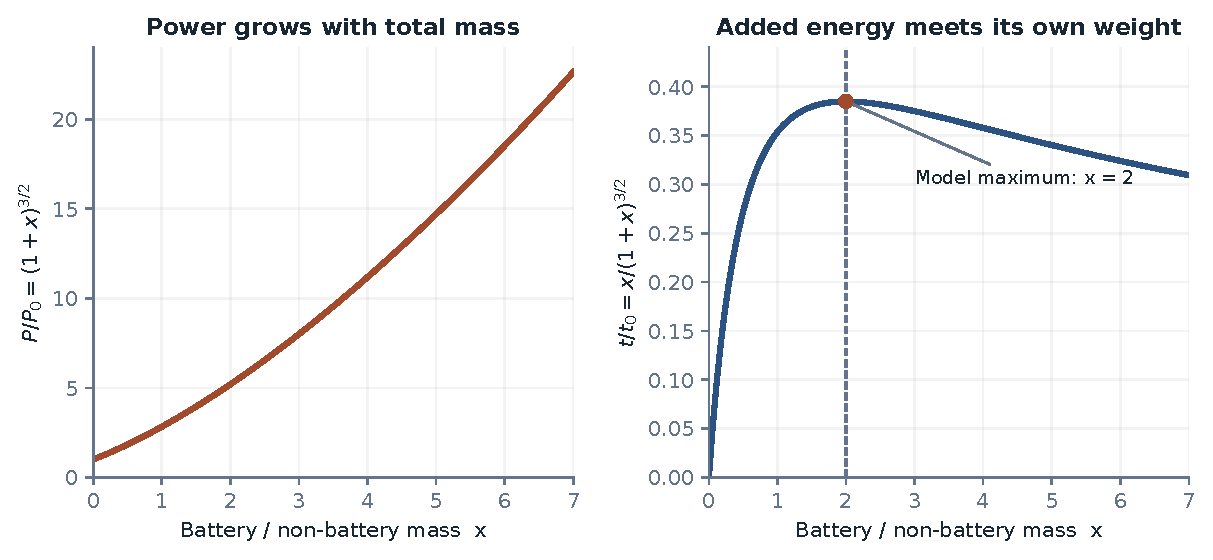
\includegraphics[width=\textwidth]{assets/hover-tradeoff.pdf}
\caption{Ideal hover at fixed disk area, air density, and efficiency. Here $x=m_b/m_0$, $P_0$ is the induced power for the non-battery mass, and $t_0=\epsilon e_bm_0/P_0$. The normalized endurance peaks at $x=2$. Structure, power limits, and mission profile add further constraints.}
\label{fig:mechanism-hover-tradeoff}
\end{figure}
